\subsection*{Anwendungen in Branchen}
Architektur: Generatives Design wird in der Architektur eingesetzt, um innovative Gebäudestrukturen zu entwerfen. Durch die Verwendung von algorithmischen Methoden und parametrischen Modellen können Architekten komplexe und effiziente Gebäudekonzepte entwickeln. Das Generative Design ermöglicht es, verschiedene Parameter wie Materialverbrauch, Energieeffizienz und Raumoptimierung zu berücksichtigen und so nachhaltige Architektur zu fördern.

Produktgestaltung: Im Bereich der Produktgestaltung eröffnet das Generative Design neue Möglichkeiten zur Entwicklung maßgeschneiderter und funktional optimierter Produkte. Durch den Einsatz von Algorithmen und automatisierten Prozessen können Designer Variationen von Produkten generieren und diese an individuelle Kundenanforderungen anpassen. Dadurch können einzigartige und effiziente Produkte mit verbesserten Leistungsmerkmalen geschaffen werden.

Automobilindustrie: In der Automobilindustrie wird das Generative Design verwendet, um leichtere und dennoch stabile Fahrzeugkomponenten zu entwickeln. Durch die Integration von algorithmischen Optimierungsmethoden können Ingenieure komplexe Strukturen gestalten, die mit herkömmlichen Designansätzen schwer umzusetzen wären. Das Ergebnis sind Fahrzeugkomponenten, die sowohl Gewicht einsparen als auch die Fahrzeugleistung verbessern, beispielsweise durch bessere Aerodynamik oder höhere strukturelle Festigkeit.

\subsection*{Generativ Design Software von Autodesk und Ablauf}

Generative Design (GD) Tools werden zunehmend in verschiedenen technischen Bereichen eingesetzt. Dabei handelt es sich um Softwaretools, die künstliche Intelligenz (KI) Methoden und Algorithmen verwenden, um Designprobleme zu lösen. Ein Unternehmen, das sich stark auf die Entwicklung solcher GD-Tools und deren Integration in herkömmliche CAD-Umgebungen konzentriert hat, ist Autodesk. Autodesk hat das Projekt "Dreamcatcher" gestartet, das sich seit 2014 der Entwicklung von GD-Tools widmet. Nach fünf Jahren Entwicklung wurde die erste Version der kommerziellen GD-Software veröffentlicht. Das GD-Tool von Autodesk heißt "Generative Design" und ist in Fusion 360, einem parametrischen CAD-Modellierer, integriert. 

Generative Design von Autodesk ermöglicht die Optimierung der Form eines Bauteils, um statische strukturelle Belastungen zu erfüllen. Cloud-Computing-Funktionen werden genutzt, um mehrere Finite-Elemente-Analysen durchzuführen und ein akzeptables Ergebnis innerhalb einer akzeptablen Zeitspanne zu erhalten. Im Gegensatz zur Topologieoptimierung erfordert Generative Design weniger Anpassungen und Einrichtungsphasen und ist somit für eine breitere Anwendung zugänglich. Dennoch erfordert die bewusste Anwendung von GD-Tools bestimmte Fähigkeiten, die derzeit noch nicht vollständig entwickelt und weit verbreitet sind. 



\begin{figure}[h]
    \begin{minipage}{0.5\textwidth}
      \centering
      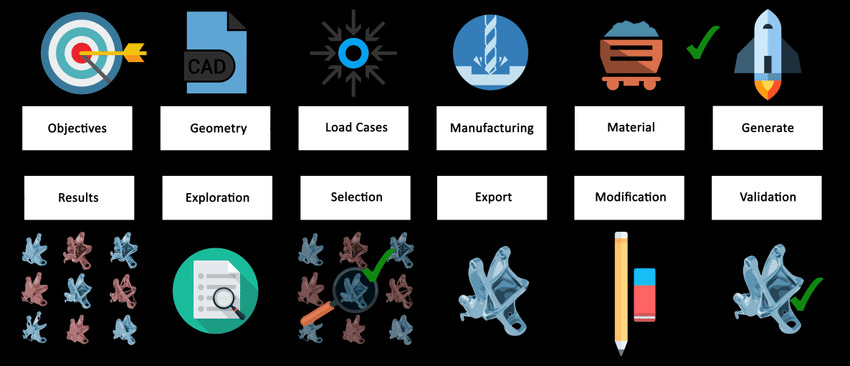
\includegraphics[width=\textwidth]{./images/Autodesk-Generative-Design-Framework.jpeg}
    \end{minipage}
    \caption{Autodesk Prozessablauf}
    \label{fig:meinbild}
  \end{figure}
  

Autodesk Generative Design bietet verschiedene Phasen im Arbeitsablauf, darunter:

1. Ziele: Der Benutzer kann zwischen zwei Optionen wählen, entweder die Masse zu minimieren oder die Steifigkeit zu maximieren. In beiden Fällen wird ein Sicherheitsfaktor benötigt. Bei Auswahl der zweiten Option muss der Benutzer auch eine Zielmasse angeben, die die Optimierung erreichen soll.

2. Geometrie: Der Benutzer definiert die Bereiche, die von der Optimierung unverändert bleiben sollen (Erhaltungsbereiche) und die Bereiche, die leer bleiben müssen (Hindernisbereiche). Im Gegensatz zum klassischen Ansatz der Topologieoptimierung erfordert Generative Design keine Definition eines Ausgangsvolumens (Designraum), das schrittweise ausgehöhlt wird. Die Optimierung kann mit einer plausiblen Ausgangsform (Starting Shape) gestartet werden, was jedoch optional ist.

3. Lastfälle: Generative Design unterstützt Kräfte, Drücke und Lagerlasten. Es können auch die Schwerkraft berücksichtigt werden. Verfügbar sind festgelegte, festgeklemmte und reibungsfreie Einschränkungen. Mehrere Lastfälle können vom Solver berücksichtigt werden, jedoch können keine dynamischen Bedingungen eingeführt werden. Alle Lasten und Einschränkungen müssen auf die Erhaltungsbereiche angewendet werden.

4. Fertigungsbeschränkungen: Der Benutzer kann Fertigungsbeschränkungen angeben, um die Optimierung auf Formen auszurichten, die mit einem bestimmten Herstellungsprozess (Additive Fertigung, 5-Achs-Fräsen, 3-Achs-Fräsen) hergestellt werden können, um die Produktionskosten für die Bauteil

fertigung zu reduzieren.

5. Material: Derzeit können nur linear-elastische Modelle verwendet werden. Generative Design ermöglicht jedoch die gleichzeitige Auswahl von bis zu zehn Materialien in einer einzigen Analyse.

6. Eingabeprüfung und Berechnung: Generative Design überprüft, ob alle erforderlichen Informationen vorhanden sind. Wenn dies der Fall ist, werden die Optimierung und die Analysen auf externen Servern mithilfe von Cloud-Computing durchgeführt, nachdem eine festgelegte Gebühr (Cloud-Credits) bezahlt wurde.

7. Ergebnisse: Sobald die Ergebnisse auf dem lokalen Computer heruntergeladen sind, stehen sie dem Benutzer zur Verfügung. Die Ergebnisse können nach mechanischen und physikalischen Eigenschaften dargestellt werden.

8. Exploration: Generative Design bietet eine dedizierte Umgebung mit Visualisierungswerkzeugen, um die Ergebnisse geordnet darzustellen und dem Benutzer bei der Identifizierung der besten Lösung zu helfen.

9. Auswahl: Der Benutzer wählt das Design aus, das am besten zu den gewünschten Anforderungen passt, und exportiert es aus der Visualisierungsumgebung.

10. Export: Das Design wird isoliert und für weitere Änderungen für den Benutzer verfügbar gemacht. Die CAD-Geometrie des Teils wird in die Modellierungsumgebung von Fusion 360 importiert. Für den Export von Designs aus der Visualisierungsumgebung fallen zusätzliche Kosten an.

11. Modifikation: Nach dem Export des Designs muss es mit herkömmlichen CAD-Tools bearbeitet werden, um Fehler zu beheben, die typischerweise in komplexen Formen mit mehreren B-REP-Oberflächen auftreten. Dies ist auch bei Topologieoptimierungen erforderlich, bei denen die tessellierten Formen, die durch die Optimierung erzeugt werden, bearbeitet und optimiert werden müssen, um die Fertigung zu ermöglichen.

12. Validierung: Die Leistungsfähigkeit der exportierten Form muss durch zusätzliche Finite-Elemente-Analysen validiert werden, um die endgültigen mechanischen Eigenschaften des Teils zu bewerten.